% Dies ist bb06.tex vom 12.02.2007 (Kr)
% Diese Datei enth�lt einen Beispieltext zum Beamer-Paket.
%  -------------------------------------------------------------------
%\documentclass[handout]{beamer}
\documentclass{beamer}

%usetheme{Boadilla}
\usetheme{Warsaw}
%\usecolortheme{rose}
%\usecolortheme{seagull}

%\usepackage{ngerman}
\usepackage[latin1]{inputenc}
\usepackage[T1]{fontenc}

\usepackage{graphicx}
\usepackage{subfigure}
\usepackage{listings}
\usepackage{url}
\usepackage{amsmath}
\usepackage{amsfonts}
\usepackage{amssymb}

%directory for graphics
\graphicspath{{gfx/}}

%\setbeamertemplate{navigation symbols}{}
%\beamertemplatesolidbackgroundcolor{black!5}
\setbeamercovered{transparent}
%  -------------------------------------------------------------------
\begin{document}
\title{Problem Set 3: KRR, CV}
\author{Benjamin Pietrowicz, Budi Yanto}
%\institute[Uni M�nster/ZIV]
%          {Westf�lische Wilhelms-Universit�t M�nster\\
%           Zentrum f�r Informationsverarbeitung}
\date{June 25, 2014}

\begin{frame}
\maketitle
\end{frame}

\newlength{\colHoehe}

\begin{frame}
\frametitle{ROC Characteristic}
	\begin{figure}[ht]
		\centering
		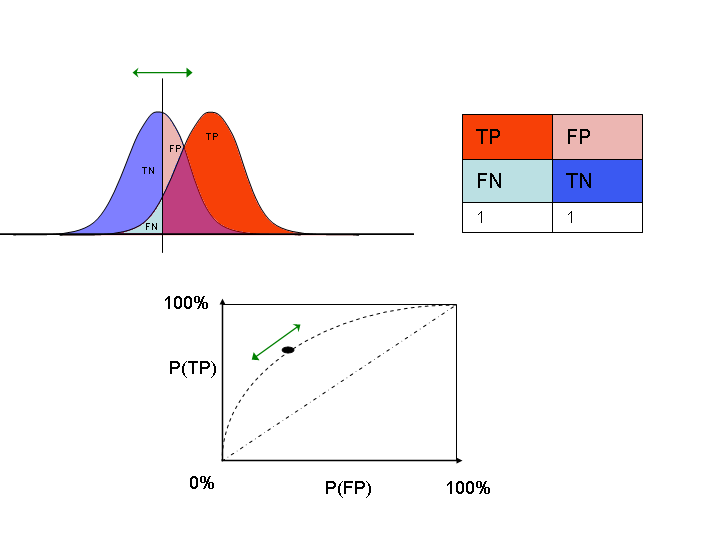
\includegraphics[scale=0.3]{ROC.png}
	\end{figure}
	Source: \url{http://en.wikipedia.org/wiki/Receiver_operating_characteristic}
\end{frame}

\begin{frame}
\frametitle{TPR, FPR}
	\begin{align*}
		TN(z) =\Phi (z-\mu_N) &\quad\quad\quad\quad FP(z) = 1-TN(z) = \Phi (\mu_n -z) \\
		FN(z) =\Phi (z-\mu_P) &\quad\quad\quad\quad TP(z) = 1-FN(z) = \Phi (\mu_p -z) \\
		TPR(z) = \cfrac{TP(z)}{TP(z)+FN(z)} &\quad\quad\quad\quad FPR(z) = \cfrac{FP(z)}{FP(z)+TN(z)}
	\end{align*}
\end{frame}

\begin{frame}
\frametitle{TPR, FPR}
	\begin{align*}
		TN(z) =\Phi (z-\mu_N) &\quad\quad\quad\quad FP(z) = 1-TN(z) = \Phi (\mu_n -z) \\
		FN(z) =\Phi (z-\mu_P) &\quad\quad\quad\quad TP(z) = 1-FN(z) = \Phi (\mu_p -z) \\
		TPR(z) = \cfrac{TP(z)}{TP(z)+FN(z)} &\quad\quad\quad\quad FPR(z) = \cfrac{FP(z)}{FP(z)+TN(z)}
	\end{align*}
	Unconditional distribution:
	\[ p(x) = p(x|y=-1) \cdot p(y=-1) + p(x|y=+1) \cdot p(y=+1)\]
\end{frame}

\begin{frame}
\frametitle{ROC Curves - 1D-Toy Data Set}
	\begin{figure}[ht]
		\centering
		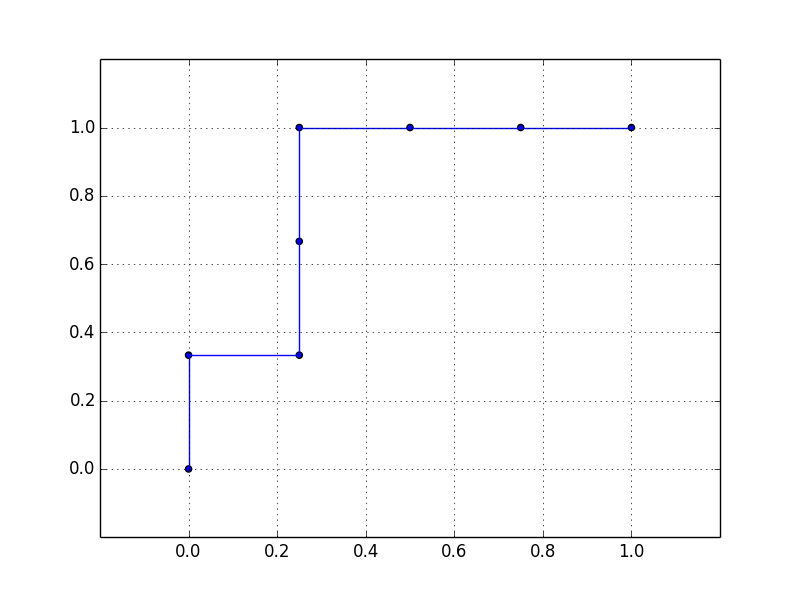
\includegraphics[scale=0.4]{emp_example.png}
	\end{figure}
	\begin{align*}
		\text{sorted samples: }-1 | +1 | -1 | -1 | +1 | +1 | +1
	\end{align*}
\end{frame}

\begin{frame}
\frametitle{ROC Curves - 1D-Toy Data Set}
	\begin{figure}[ht]
		\centering
		\mbox{
			\subfigure{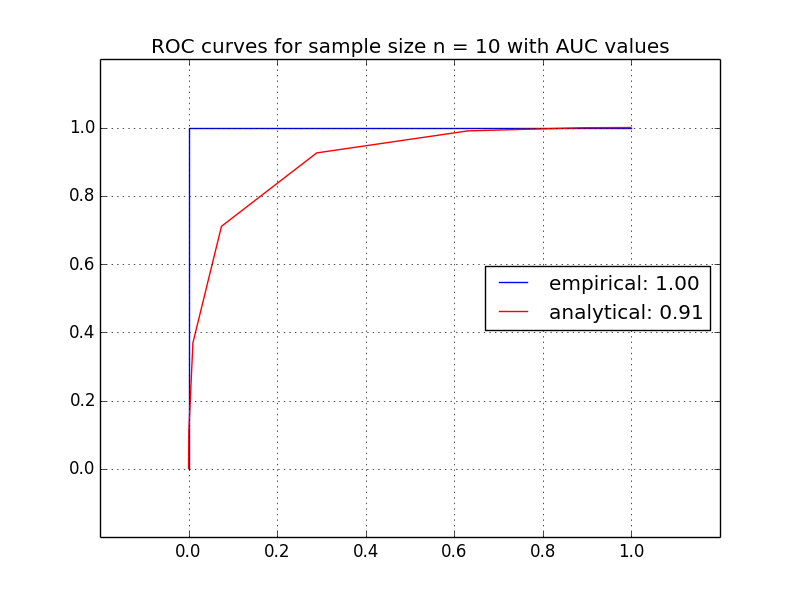
\includegraphics[scale=0.25]{figure_1.png} }\quad
			\subfigure{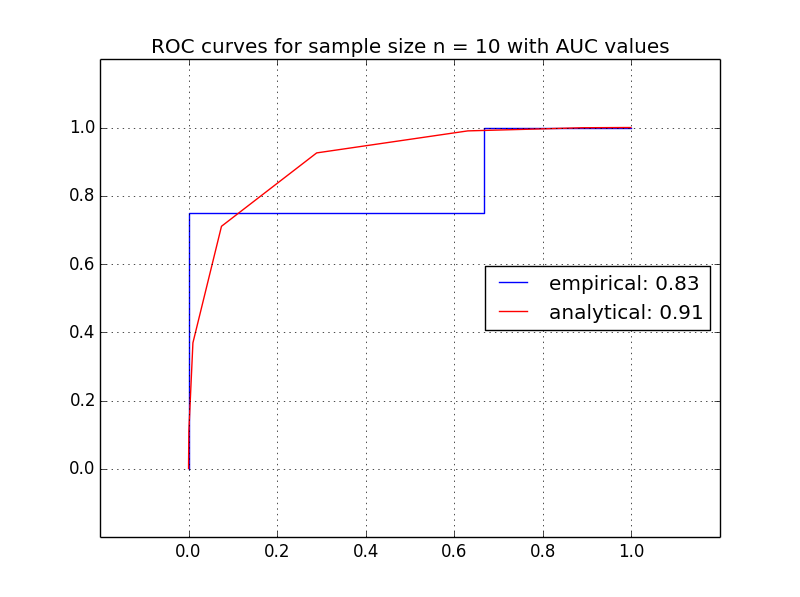
\includegraphics[scale=0.25]{figure_1b.png} }}
			\caption{ROC curves for sample size n = 10}
	\end{figure}
\end{frame}

\begin{frame}
\frametitle{ROC Curves - 1D-Toy Data Set}
	\begin{figure}[ht]
		\centering
		\mbox{
			\subfigure{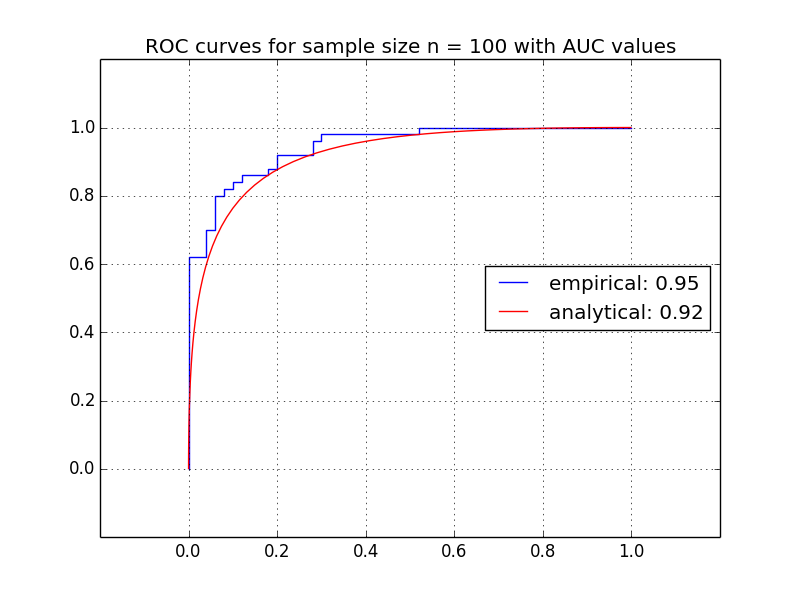
\includegraphics[scale=0.25]{figure_2.png} }\quad
			\subfigure{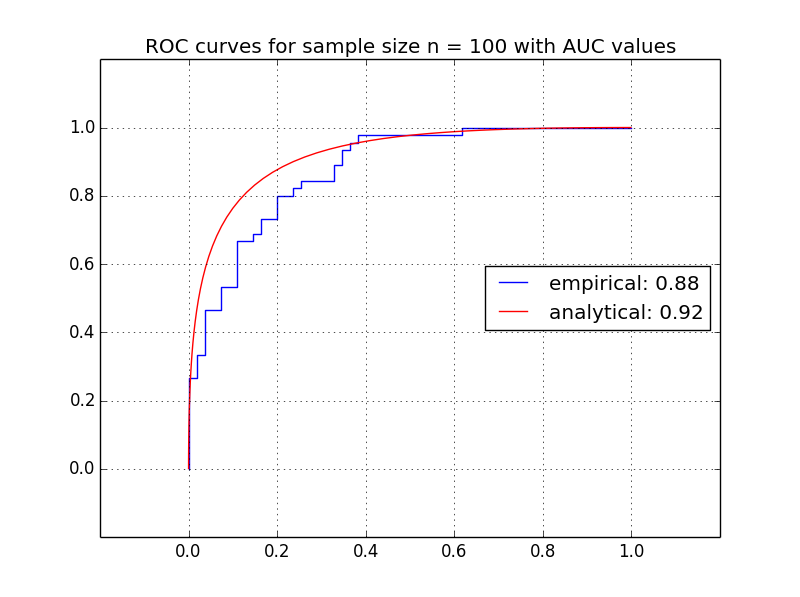
\includegraphics[scale=0.25]{figure_2b.png} }}
			\caption{ROC curves for sample size n = 100}
	\end{figure}
\end{frame}

\begin{frame}
\frametitle{ROC Curves - 1D-Toy Data Set}
	\begin{figure}[ht]
		\centering
		\mbox{	
			\subfigure{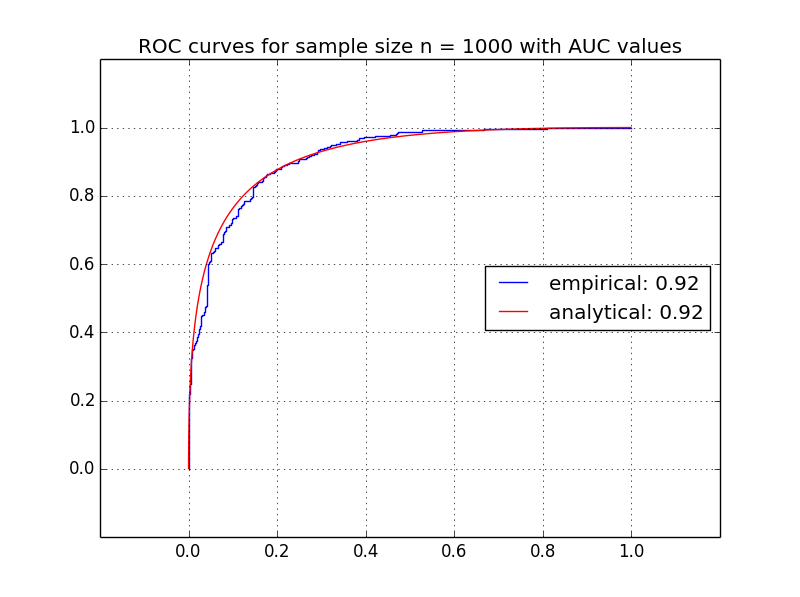
\includegraphics[scale=0.25]{figure_3.png} }\quad
			\subfigure{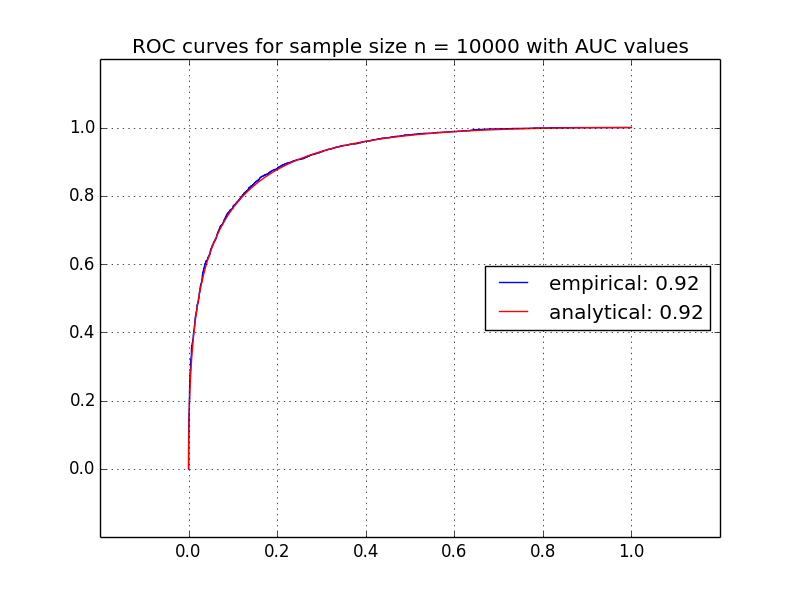
\includegraphics[scale=0.25]{figure_4.png} }}
			\caption{ROC curves for sample size n = 1000 and n = 10000}
	\end{figure}
\end{frame}

\begin{frame}
\frametitle{Data Sets}
	\centering
	\begin{table}
	\begin{tabular}{l*{6}{c}r}
	\textbf{Data Set}         & \textbf{Dimension} & \textbf{Total Training Data} & \textbf{Total Test Data}\\
	\hline
	Banana & 2 & 400 & 4900  \\
	Diabetis            & 8 & 468 & 300  \\
	Flare-Solar           & 9 & 666 & 400  \\
	Image     & 18 & 1300 & 1010 \\
	Ringnorm     & 20 & 400 & 7000 \\
	\end{tabular}
	\end{table}
\end{frame}

\begin{frame}
\frametitle{Cross-Validation Parameters}
	\centering
	\begin{itemize}
		\item \textbf{Cross-Validation} with $nrepetitions=2$ and $nfolds=10$
		\item \textbf{LOOCV}: regularization = [0]
  \end{itemize}
	
	\begin{table}
	\begin{tabular}{l*{6}{l}r}
	\textbf{Kernel}         & \textbf{Kernel Parameters} & \textbf{Regularization}\\
	\hline
	Linear & [0] & np.logspace(-2,2,10)  \\
	Polynomial     & np.arange(1,10) & np.logspace(-2,2,10)  \\
	Gaussian           & np.logspace(-2,2,10) & np.logspace(-2,2,10)  \\
	\end{tabular}
	\end{table}
\end{frame}

\begin{frame}
\frametitle{Cross-Validation Results}
	\centering
	\begin{table}
	\begin{tabular}{l*{6}{c}r}
	\textbf{Data Set}  & \textbf{Kernel} & \textbf{Parameter} & \textbf{Regularization} & \textbf{Cvloss} \\
	\hline
	Banana & Gaussian & 0.215 & 2.154 & 0.096\\
	Diabetis  & Gaussian & 4.642 & 2.154 & 0.237 \\
	Flare-Solar  & Polynomial & 2.0 & 762.223 & 0.347 \\
	Image     & Gaussian & 0.599 & 0.464 & 0.028 \\
	Ringnorm     & Gaussian & 4.642 & 0.464 & 0.062\\
	\end{tabular}
	\caption{LOOCV}
	\end{table}
	
	\begin{table}
	\begin{tabular}{l*{6}{c}r}
	\textbf{Data Set}  & \textbf{Kernel} & \textbf{Parameter} & \textbf{Regularization} & \textbf{Cvloss}\\
	\hline
	Banana & Gaussian & 0.215 & 4.642 & 0.096\\
	Diabetis  & Gaussian & 35.938 & 0.010 & 0.241\\
	Flare-Solar  & Gaussian & 35.938 & 0.010 & 0.348 \\
	Image     & Gaussian & 1.668 & 0.028 & 0.022 \\
	Ringnorm     & Gaussian & 4.642 & 0.077 & 0.039\\
	\end{tabular}
	\caption{Standard CV}
	\end{table}
\end{frame}


\begin{frame}
\frametitle{ROC Curves - Banana}
	\begin{figure}[ht]
		\centering
		\mbox{
			\subfigure{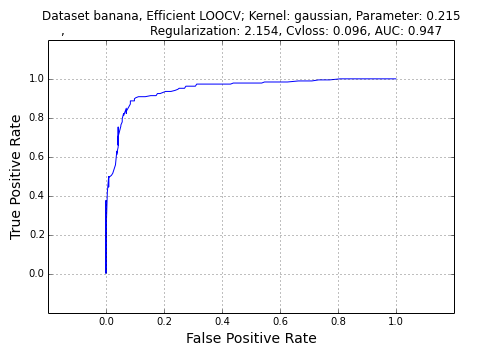
\includegraphics[scale=0.3]{roc_curve_banana_loocv.png} }\quad
			\subfigure{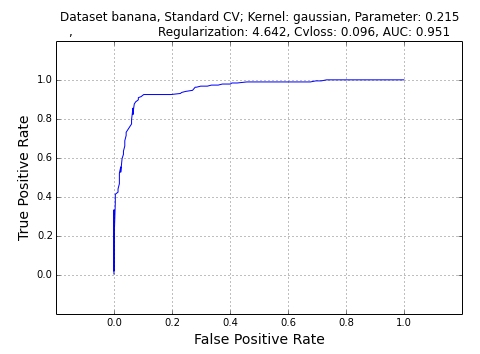
\includegraphics[scale=0.3]{roc_curve_banana_cv.png} }}
			\caption{ROC curves of banana dataset}
	\end{figure}
\end{frame}

\begin{frame}
\frametitle{ROC Curves - Diabetis}
	\begin{figure}[ht]
		\centering
		\mbox{
			\subfigure{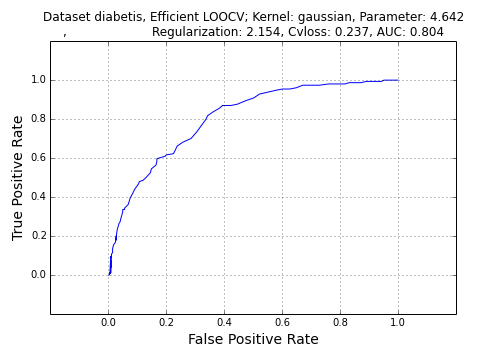
\includegraphics[scale=0.3]{roc_curve_diabetis_loocv.png} }\quad
			\subfigure{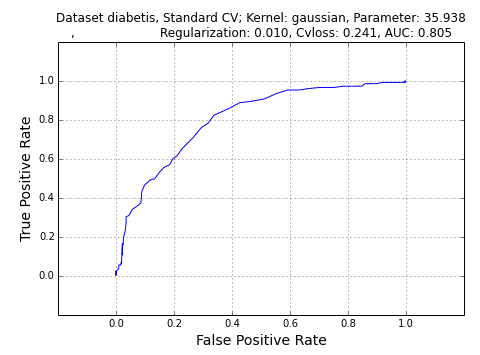
\includegraphics[scale=0.3]{roc_curve_diabetis_cv.png} }}
			\caption{ROC curves of diabetis dataset}
	\end{figure}
\end{frame}

\begin{frame}
\frametitle{ROC Curves - Flare-Solar}
	\begin{figure}[ht]
		\centering
		\mbox{
			\subfigure{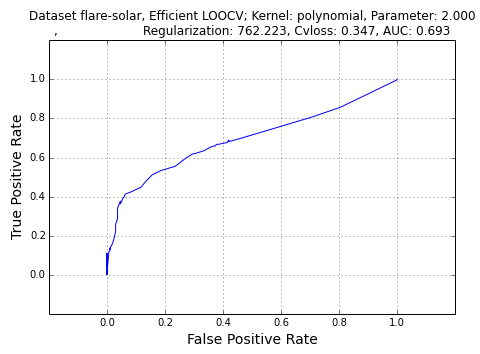
\includegraphics[scale=0.3]{roc_curve_flare_solar_loocv.png} }\quad
			\subfigure{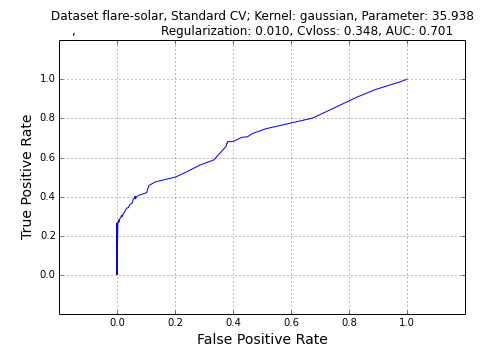
\includegraphics[scale=0.3]{roc_curve_flare_solar_cv.png} }}
			\caption{ROC curves of flare-solar dataset}
	\end{figure}
\end{frame}

\begin{frame}
\frametitle{ROC Curves - Image}
	\begin{figure}[ht]
		\centering
		\mbox{
			\subfigure{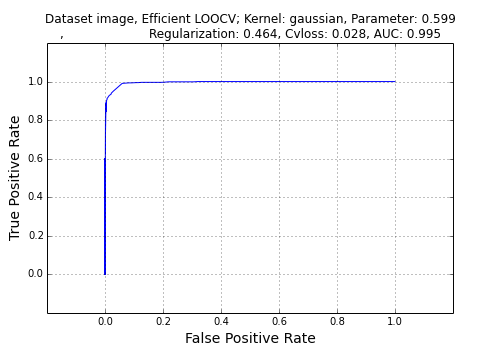
\includegraphics[scale=0.3]{roc_curve_image_loocv.png} }\quad
			\subfigure{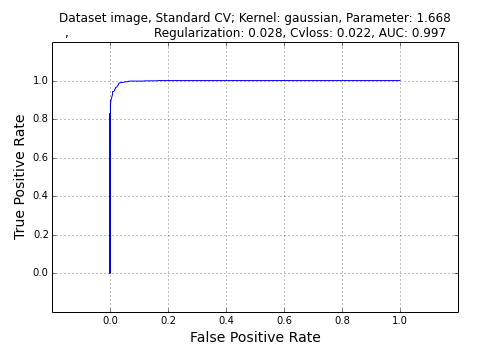
\includegraphics[scale=0.3]{roc_curve_image_cv.png} }}
			\caption{ROC curves of image dataset}
	\end{figure}
\end{frame}

\begin{frame}
\frametitle{ROC Curves - Ringnorm}
	\begin{figure}[ht]
		\centering
		\mbox{
			\subfigure{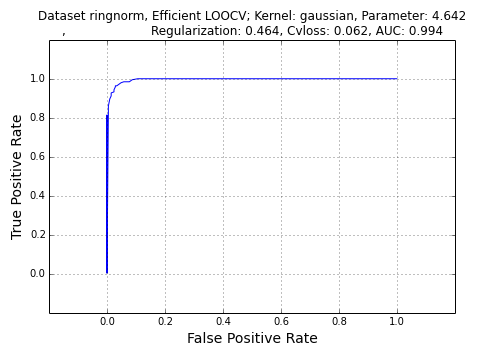
\includegraphics[scale=0.3]{roc_curve_ringnorm_loocv.png} }\quad
			\subfigure{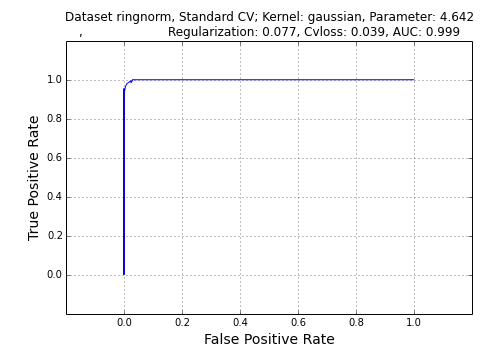
\includegraphics[scale=0.3]{roc_curve_ringnorm_cv.png} }}
			\caption{ROC curves of ringnorm dataset}
	\end{figure}
\end{frame}


\begin{frame}
\frametitle{Correspondence between Cvloss and AUC}
	\begin{figure}[ht]
		\centering
		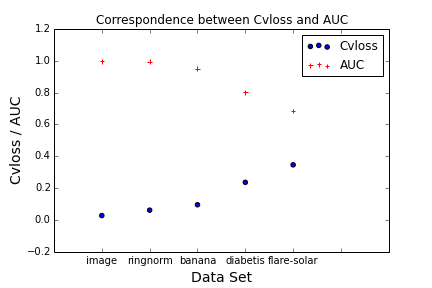
\includegraphics[scale=0.5]{cvloss_auc.png}
		\caption{Correspondence between Cvloss and AUC}
	\end{figure}
\end{frame}

\begin{frame}
\frametitle{Comparison of Standard CV and LOOCV}
	\centering
	\begin{table}
	\begin{tabular}{l*{6}{c}r}
	\textbf{Data Set}  & \textbf{Cvloss LOOCV} & \textbf{Cvloss St. CV} \\
	\hline
	Banana & 0.096 & 0.096\\
	Diabetis  & 0.237 & 0.241 \\
	Flare-Solar  & 0.347 & 0.348 \\
	Image     & 0.028 & 0.022 \\
	Ringnorm     & 0.062 & 0.039 \\
	\end{tabular}
	\end{table}
	
	\begin{table}
	\begin{tabular}{l*{6}{c}r}
	\textbf{Data Set}  & \textbf{Time LOOCV (in sec.)} & \textbf{Time St. CV (in sec.)} \\
	\hline
	Banana & 109.220 & 78.326 \\
	Diabetis  & 237.252 & 113.388 \\
	Flare-Solar  & 466.499 & 217.701 \\
	Image     & 4596.275 & 1420.264 \\
	Ringnorm     & 126.286 & 96.347\\
	\end{tabular}
	\end{table}
\end{frame}

\begin{frame}
	\begin{center}
		\Huge \textbf{Thank you !!!}
	\end{center}
\end{frame}

\end{document}

